\section{Artefact Design}\label{sec:chapter-5}

\subsection{System architecture}

The mobile application communicates with the Node API, which authenticates requests and coordinates persistence, content access, and recommendation generation. The API queries PostgreSQL for account-specific context and published recommendable exercises, maps comfort choices to constraints, pseudonymises interaction identifiers, and calls the Python service. Returned items are recorded and exposed through the application. The administrator uses protected content endpoints and signed media-upload operations. Figure~\ref{fig:architecture} separates these responsibilities and shows the journal boundary alongside the ordinary application data flow.

Keeping the recommender behind the API prevents the mobile client from directly deciding another account's context. PostgreSQL provides relationships and transaction support; object storage handles media delivery separately. A signed URL grants a bounded storage operation without distributing permanent storage credentials to the client. These are design mechanisms rather than evidence of a completed security audit. Service configuration, deployment policies, and operational logging must preserve the same boundaries in a release environment.

\begin{figure}[htbp]
\centering
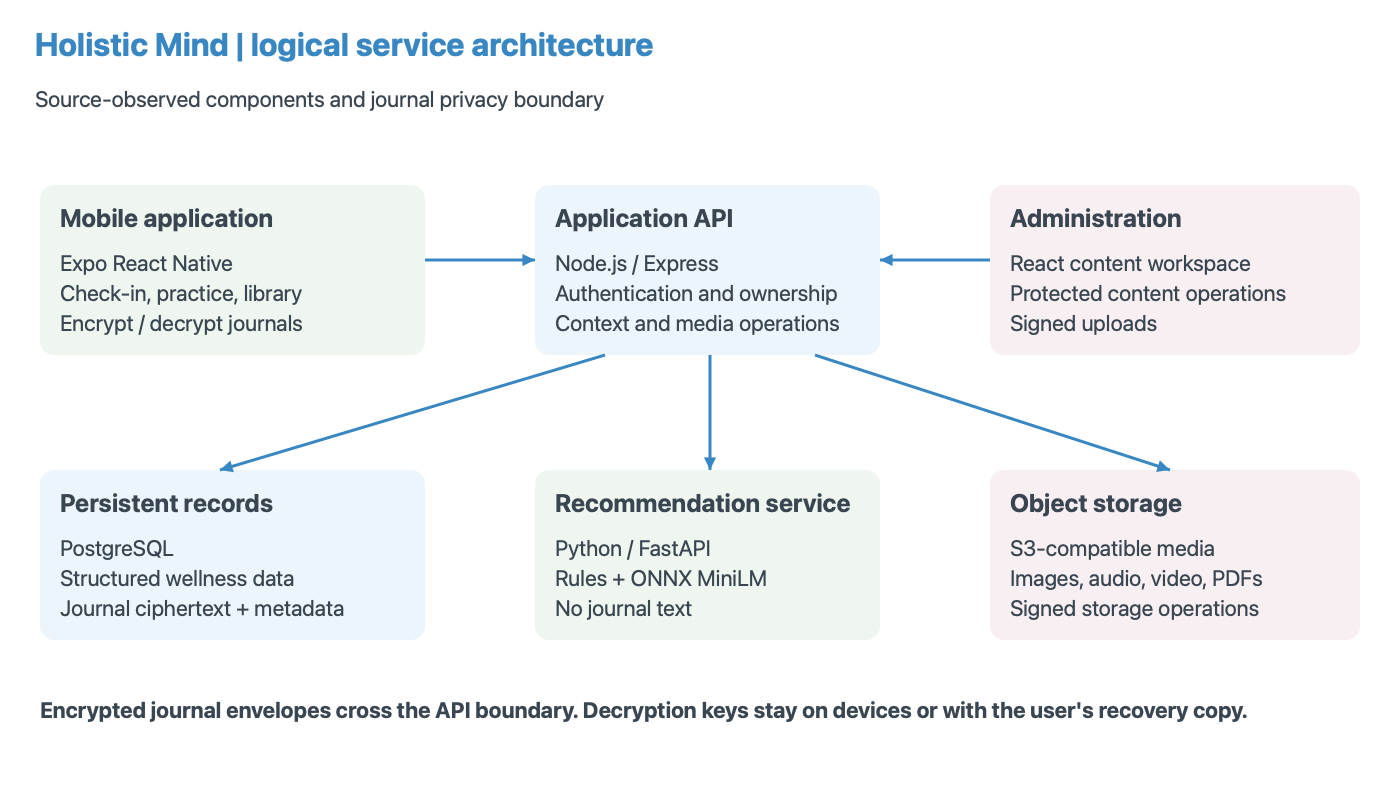
\includegraphics[width=\linewidth,height=0.62\textheight,keepaspectratio]{figures/architecture.png}
\caption[Logical service architecture]{Current logical architecture reconstructed from source. Journal content is encrypted before upload; structured wellness context reaches the separate recommendation service.}
\label{fig:architecture}
\end{figure}
\FloatBarrier

\subsection{User journey and interface design}

The user journey begins with welcome, account access, and brief onboarding. The Home screen prioritises daily check-in and relevant next actions. Explore offers user-led browsing, Journal provides reflective writing, Library organises learning content, and Profile manages account-related settings. History presents previous activity and check-in information. This arrangement gives personalisation a clear place without requiring every activity to start from a recommendation.

The visual design uses warm neutral backgrounds, rounded components, body-based illustrations, and restrained accent colours. Selected states, readable spacing, and short prompts aim to reduce interaction complexity. Figure~\ref{fig:journey} shows the daily loop, while Figure~\ref{fig:library} later illustrates the implemented library screen. These observations describe design intent. Without measured task completion, accessibility testing, or participant feedback, the report cannot conclude that the interface is easy for every target user.

\begin{figure}[htbp]
\centering
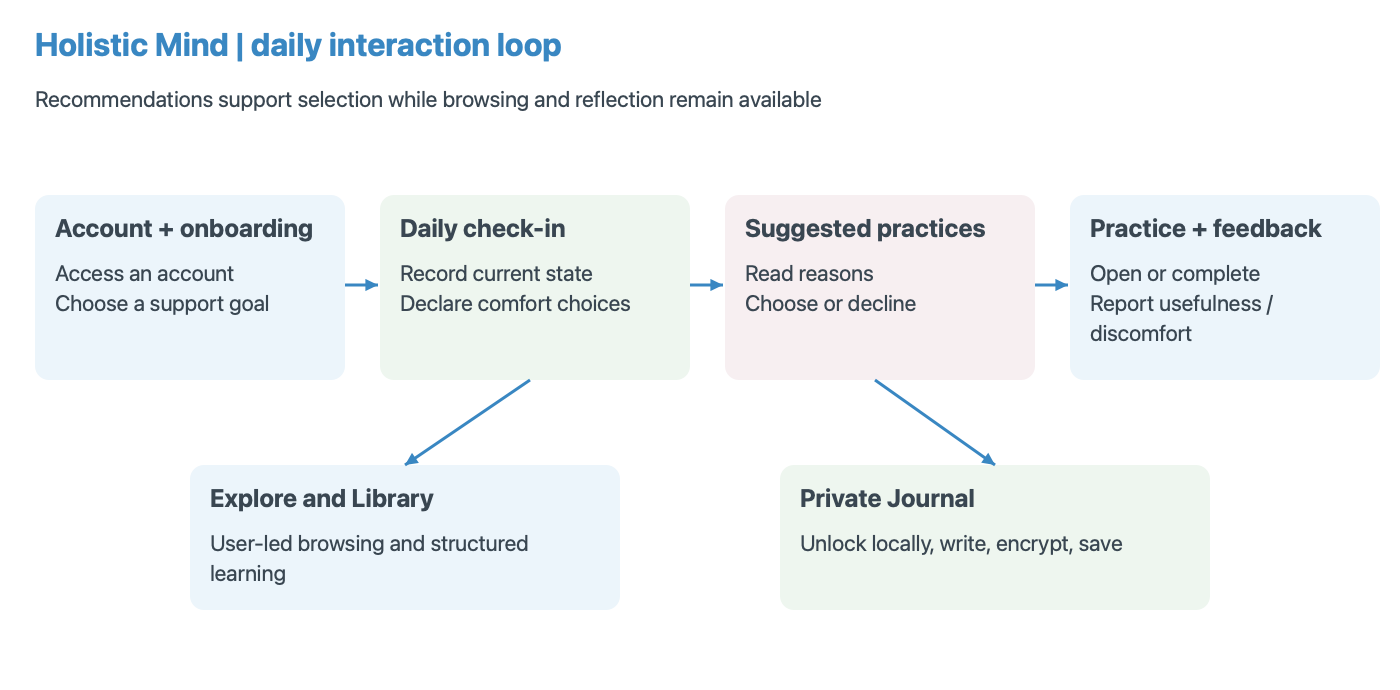
\includegraphics[width=\linewidth,height=0.62\textheight,keepaspectratio]{figures/journey.png}
\caption[Daily user journey]{Daily user journey. Browsing and encrypted reflection remain voluntary parallel paths; practice feedback contributes to later recommendations.}
\label{fig:journey}
\end{figure}
\FloatBarrier

A practical example clarifies the interaction. A user reports feeling scattered and selects focus as the immediate support need. If the same user also avoids breath holds, the recommendation pathway must remove exercises requiring that action before deciding which remaining practice best matches focus. The interface should present the resulting options as suggestions with reasons, and the user may still choose another activity through Explore. Reporting discomfort provides additional evidence for future exclusions. This example illustrates the intended sequence, not a new measured test case or a claim about the user's eventual response to a practice.

\subsection{Data model and ownership}

Private records are associated with a server-established user identity. The principal groups include accounts and profiles, authentication sessions, onboarding responses, daily check-ins, encrypted journal entries and vault records, recommendation requests and items, and interaction feedback. Content groups include exercises, media, courses, modules, and related learning resources. Figure~\ref{fig:data} presents a simplified relationship map; it deliberately omits operational columns and is not a substitute for the actual migration definitions.

Ownership matters especially when reading journals, retrieving history, or submitting recommendation feedback. Knowing an object identifier should not grant access to another account's record. Recommendation feedback is tied to an exercise returned in an owned request. The journal API validates versioned envelopes while deriving the account from authentication. These checks complement database relationships: a schema can express associations, but application queries must still apply account boundaries consistently.

\begin{figure}[htbp]
\centering
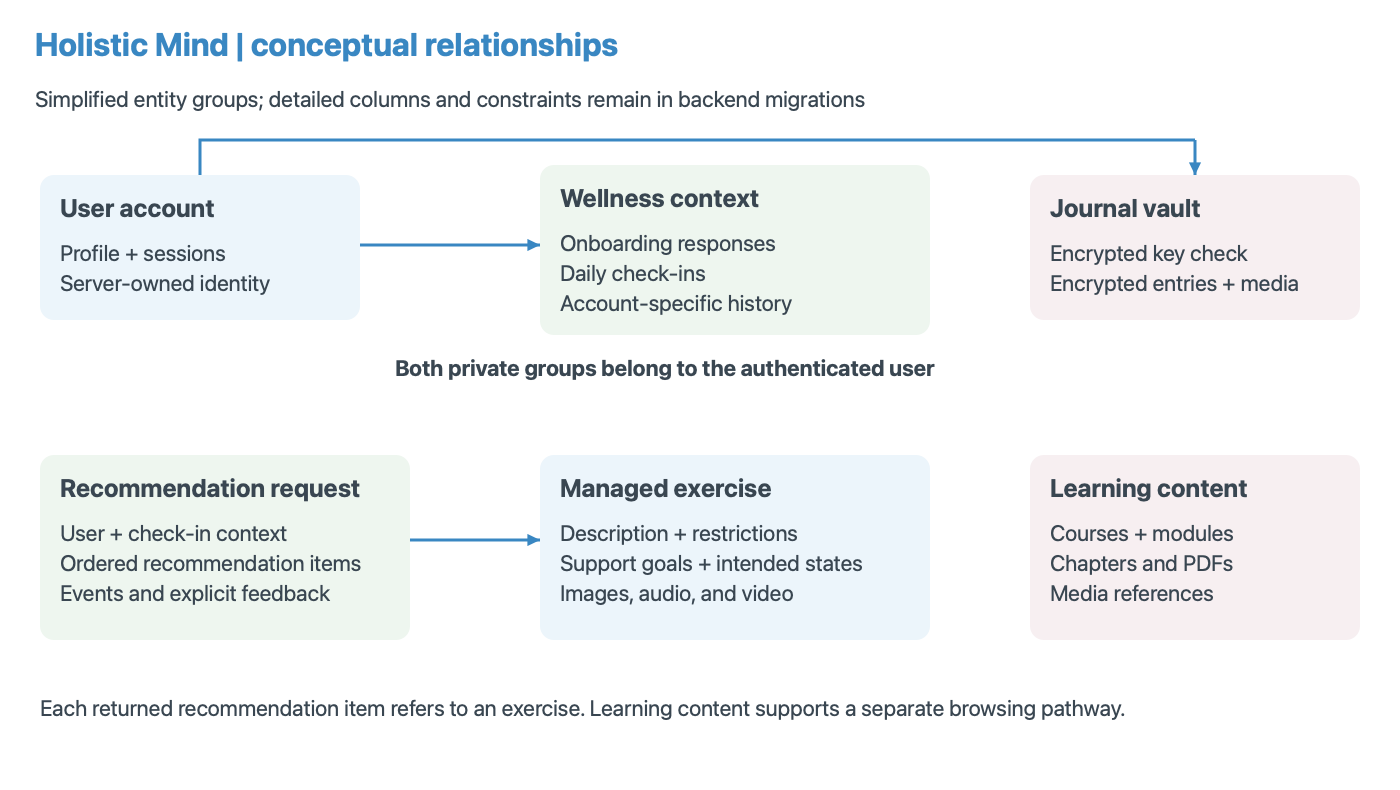
\includegraphics[width=\linewidth,height=0.62\textheight,keepaspectratio]{figures/data.png}
\caption[Conceptual data relationships]{Simplified conceptual data relationships. Private wellness records belong to users; recommendation items refer to managed exercise content.}
\label{fig:data}
\end{figure}
\FloatBarrier

\subsection{Recommendation pipeline}

The pipeline first constructs eligible candidates using known contraindications and explicit exclusions. It then builds text documents from current check-in answers, the onboarding goal, and exercise metadata. The current application sends an empty journal list. After tokenisation and ONNX inference, normalised embeddings support cosine-based comparison. Structured rules assess alignment with declared needs. Collaborative evidence is considered only when interaction overlap and neighbour thresholds are met. This sequencing prevents a filtered exercise from re-entering through a later scoring component.

In cold start, the base score is S = 0.72R + 0.23C + 0.05H, where R represents rules, C current-context similarity, and H goal/\allowbreak{}history similarity. When collaboration is active, S = 0.65R + 0.20C + 0.05H + 0.10B, with B the collaborative component. The engine subtracts recency penalties and uses category diversity during selection. Primary-support alignment and a limited fresh-item substitution may also shape the final list. Consequently, a returned position is not simply a sorted semantic score.

\begin{figure}[htbp]
\centering
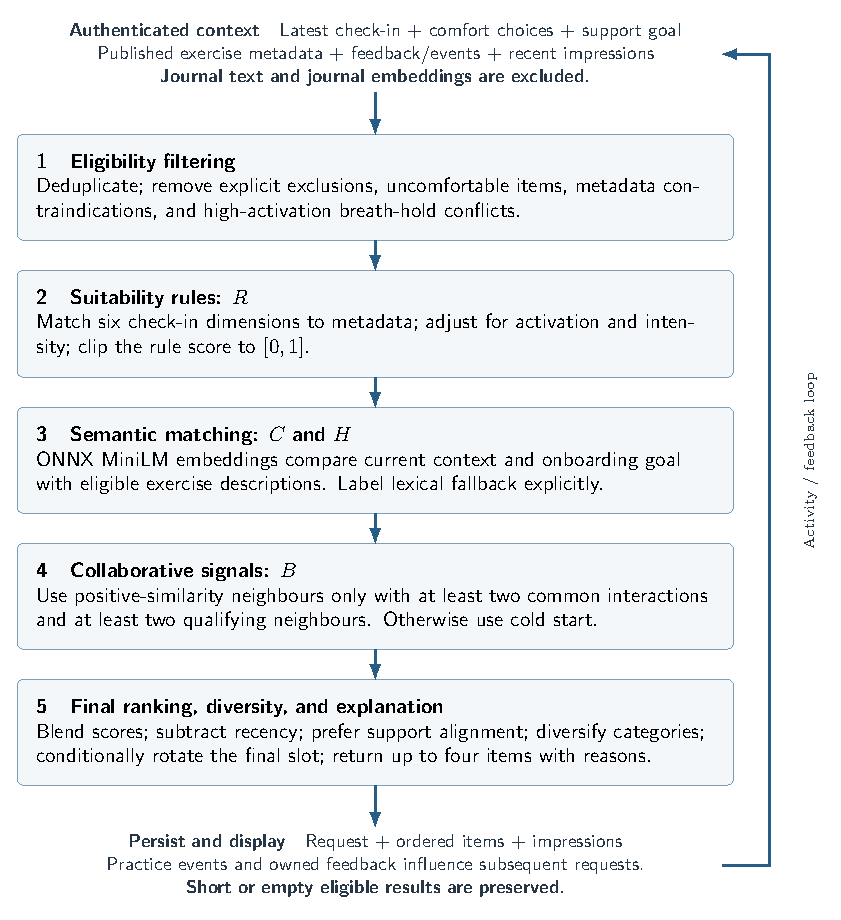
\includegraphics[width=\linewidth,height=0.70\textheight,keepaspectratio]{figures/recommendation-five-stages.pdf}
\caption[Five-stage recommendation engine and feedback loop]{The five-stage recommendation engine and feedback loop. Eligibility is enforced before any scoring; journal text and embeddings are excluded from current application requests.}
\label{fig:recommendation-five-stages}
\end{figure}
\FloatBarrier

\subsection{Privacy design}

Journal content uses a separate trust boundary from recommendations. A device generates a random 256-bit key, encrypts entry content using XChaCha20-Poly1305 with a fresh 24-byte nonce, and uploads an authenticated envelope. Associated data binds encryption to identifiers and purpose. Native key storage uses account-scoped SecureStore; web unlocks keep the key in memory. Recovery imports the user's recovery key and verifies an encrypted known value. Figure~\ref{fig:privacy} shows how persistent storage can coexist with device-side decryption.

The server can still observe ownership, timestamps, counts, identifiers, and ciphertext lengths. Check-ins, comfort choices, and feedback also remain readable to application services. Losing every device key and recovery copy makes encrypted entries unrecoverable. Ordinary account-password reset does not restore journal access. Existing plaintext entries require an explicit migration path, and clearing current database fields does not erase earlier backups. These limits are essential to describing what the privacy design actually protects.

\subsection{Relational modelling and consistency}

The database design builds on a clear separation between account identity, private activity, content, and recommendation evidence. A user row provides the ownership reference for profiles, sessions, onboarding, check-ins, journals, and recorded practice. Managed content has its own identifiers and publication lifecycle. Recommendation requests retain model version and context, while returned items preserve position, score components, reason, and exploration status. This supports a later explanation of which engine produced a displayed result.

Several source-defined constraints make application assumptions explicit. Email addresses are unique and normalised. Check-ins are unique per user and date, allowing a same-day update without creating multiple daily records. Recommendation items are unique within a request and occupy distinct positions. Feedback values have bounded helpfulness and enumerated state-change fields. Foreign-key cascades support deletion of user-linked data, but records outside the application database, such as retained exports or copied recovery keys, require separate handling.

PostgreSQL's JSONB fields accommodate variable answer and envelope structures without abandoning relational ownership. Arrays store exercise tags and goals, while constraints restrict activation and intensity values. This is a more appropriate account of flexibility than assuming every varying field requires a document database. The Modern Data Stores coursework provides a useful precedent for matching storage to workload, but Holistic Mind does not implement that coursework's MongoDB replica set or MQTT ingestion.

Indexes correspond to frequent access patterns: user-and-date lookup for check-ins, user-and-created-time retrieval for reflections and practice events, and publication-order lookup for exercises and courses. Their existence is source evidence, not a measured database-performance result. A future load test should inspect query plans and concurrency under realistic catalogue and account volumes. Small local datasets cannot establish the scaling behaviour of a deployed service.

\subsection{API contracts and sequence design}

A recommendation request is a coordinated sequence rather than a direct model call. Authentication establishes the user. The Node route loads the latest check-in and published recommendable content, derives restrictions, aggregates interactions, and prepares a pseudonymous context. The Python response identifies the model and strategy and supplies up to the requested number of items. The Node layer records the request and items, allowing subsequent events and feedback to be tied to what was actually returned. Figure~\ref{fig:sequence} summarises this sequence.

\begin{figure}[htbp]
\centering
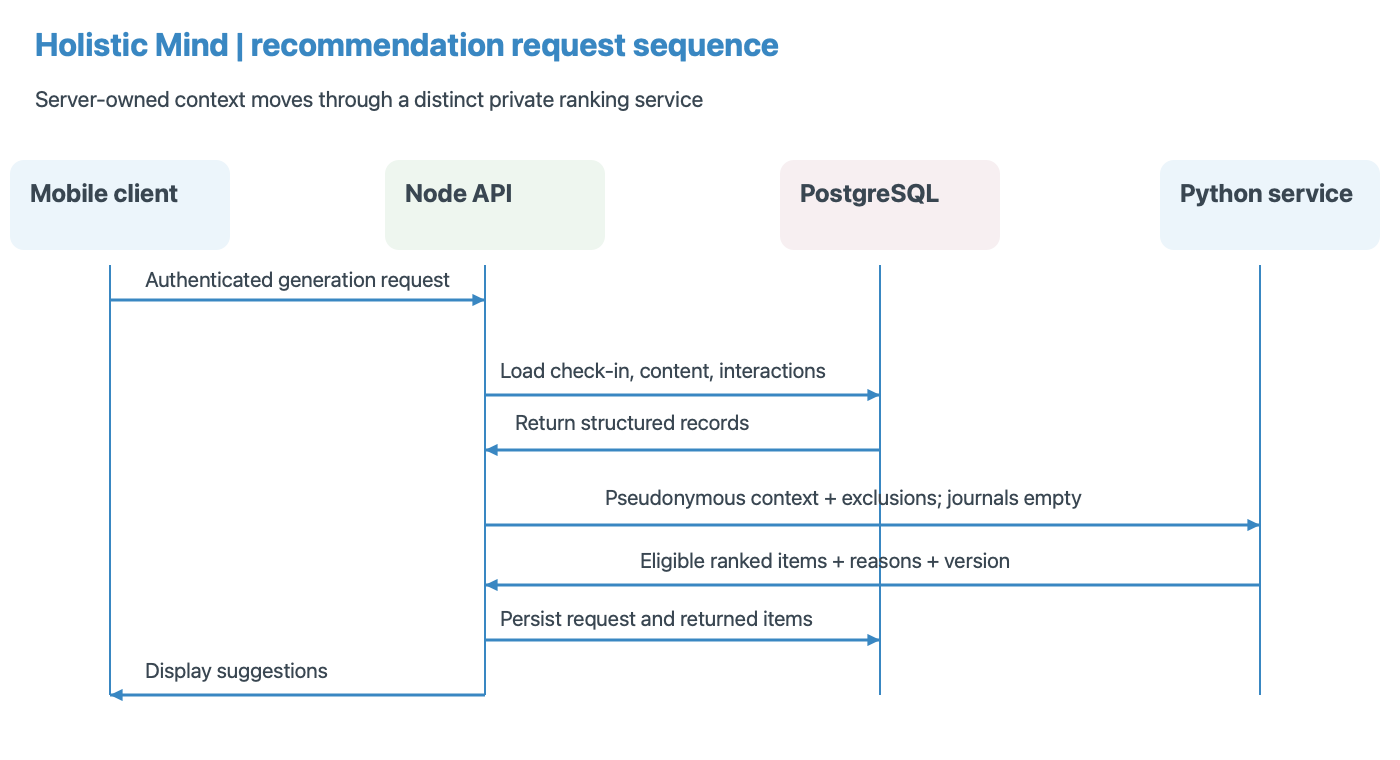
\includegraphics[width=\linewidth,height=0.62\textheight,keepaspectratio]{figures/sequence.png}
\caption[Recommendation API sequence]{Source-grounded recommendation request sequence, including authentication, contextual queries, constrained ranking, and persistence of returned items.}
\label{fig:sequence}
\end{figure}
\FloatBarrier

The contract has meaningful error states. A missing check-in prevents recommendation generation rather than permitting the client to fabricate server context. An unavailable published catalogue differs from an eligible set emptied by restrictions. A service failure may activate the application's separate fallback, while a successful empty result must remain empty. Each state has a different user-facing implication and should remain distinguishable in integration tests.

Journal operations have a different contract. Vault creation stores an encrypted check value, new entry writes accept envelopes, and normal reads return encrypted entries. A dedicated legacy path exposes older records only to the authenticated owner for migration. Media operations validate account and entry relationships. Separating these routes helps the interface explain whether it needs login, journal unlock, recovery material, or a retry of the network operation. A single generic save failure would obscure those distinctions.

\subsection{Media and publication lifecycle}

The content pipeline separates record creation from media upload and publication. An administrator requests a signed upload, transfers the asset to S3-compatible storage, and associates its reference with the appropriate record. Media and catalogue states distinguish drafts from ready or published content. The current upload helpers use a fifteen-minute expiry. A valid signed operation does not guarantee that the resulting media is correctly encoded or that its associated guidance has been reviewed, so readiness checks remain necessary.

Learning resources may be public or publicly retrievable according to deployment configuration, while encrypted journal attachments follow a different API and storage path. The existence of public educational media should not lead to treating private reflection as another content upload. The administrator's content-promotion scripts also have a different purpose from a backup of account data. These distinctions are inherited from the project's final progress review and made more explicit in the current design.
